
\chapter{Definitions}
\label{cha:definitions}

\section{Development Process of a Software Project}
When you have to make a software project plan, you have to define the main requirements that achieve the main goals of the business idea within the software project realization motivation. First, you have to define the functional requirements. In software engineering, functional requirements define the main features of each software component involved in the project. Requirements like design, basic functionalities, and defined flows are built on the functional requirements definition process.
After that, you have to define the main requirements that do not directly impact the user experience, which are called non-functional requirements. Non-functional requirements indirectly affect your software project; bad planning about those requirements could progressively affect the user performance and the software project architecture, becoming slower, heavier, or less useful for a single application user. In this process, you must design a solution that satisfies the functional and non-functional requirements. This process is called the design process of a software project. Inside this stage, you must define the number of components that give the software its functionalities. Furthermore, you have to each component infrastructure into a process named Software Architecture Definition \citet{software-engineering-book}.  The software development process involves some steps: 

\subsection{Discovery}
This stage consists of the definition of the main features of the software application. The discovery process defines the objective of the application and its main requirements. Furthermore, this gives an initial version of the behavior and the design of the software application.

\subsection{Design}
After the discovery of the application requirements, it is possible to define the design of the components of the software application and their relationships. In this stage, we define the functional and non-functional requirements. The functional requirements define the main features and use cases of the software application, defining a complete flow with the final user. The non-functional requirements define the performance metrics that the application must achieve. Based on the ISO rule, which defines the quality assurance of any software application. There is a set of defined non-functional requirements categories for achieving good performance in a software application: Scalability, availability, security, latency, integration capacity, and modification capacity (We will talk about these categories later). Once the prioritized non-functional requirements are defined, we define the rules and standards that will manage the performance of the software application.

\subsection{Development}
With the initial design of the software application and its components, we can implement and develop the software application. With a bad design process or a bad development process, it is possible to generate a deviation from the initial design of the application or a violation according to the initially defined standards of the software application.

\subsection{Testing and Quality Assurance (QA)}
With the design of the software application and its implementation, it is possible to test the main features and flows based on the designed use cases of the software application. In this stage, it would report code smells or bad performance metrics, according to the prioritized non-functional requirements.

\subsection{Release}
Once the application is tested, it achieves its performance metrics. The software application deploys in a production environment, with the final users' direct interaction. If the design process or the development process is implemented badly, it would affect the user performance of any software application. Focused on Android application development, the user experience would decay significantly, decreasing the number of active users or increasing the resources used in Android devices as the main consequences.

\subsection{Maintenance}
After the release and deployment stage. For a guarantee of the application's sustainability. It should create a refactoring process. That process consists of libraries updating, code smells fixing, and fixing bad design or development issues. The costs of one software application in terms of human resources, time, and money could increase the time goes by if the latest stages are implemented badly.

\begin{figure}[h]
    	\centering
    		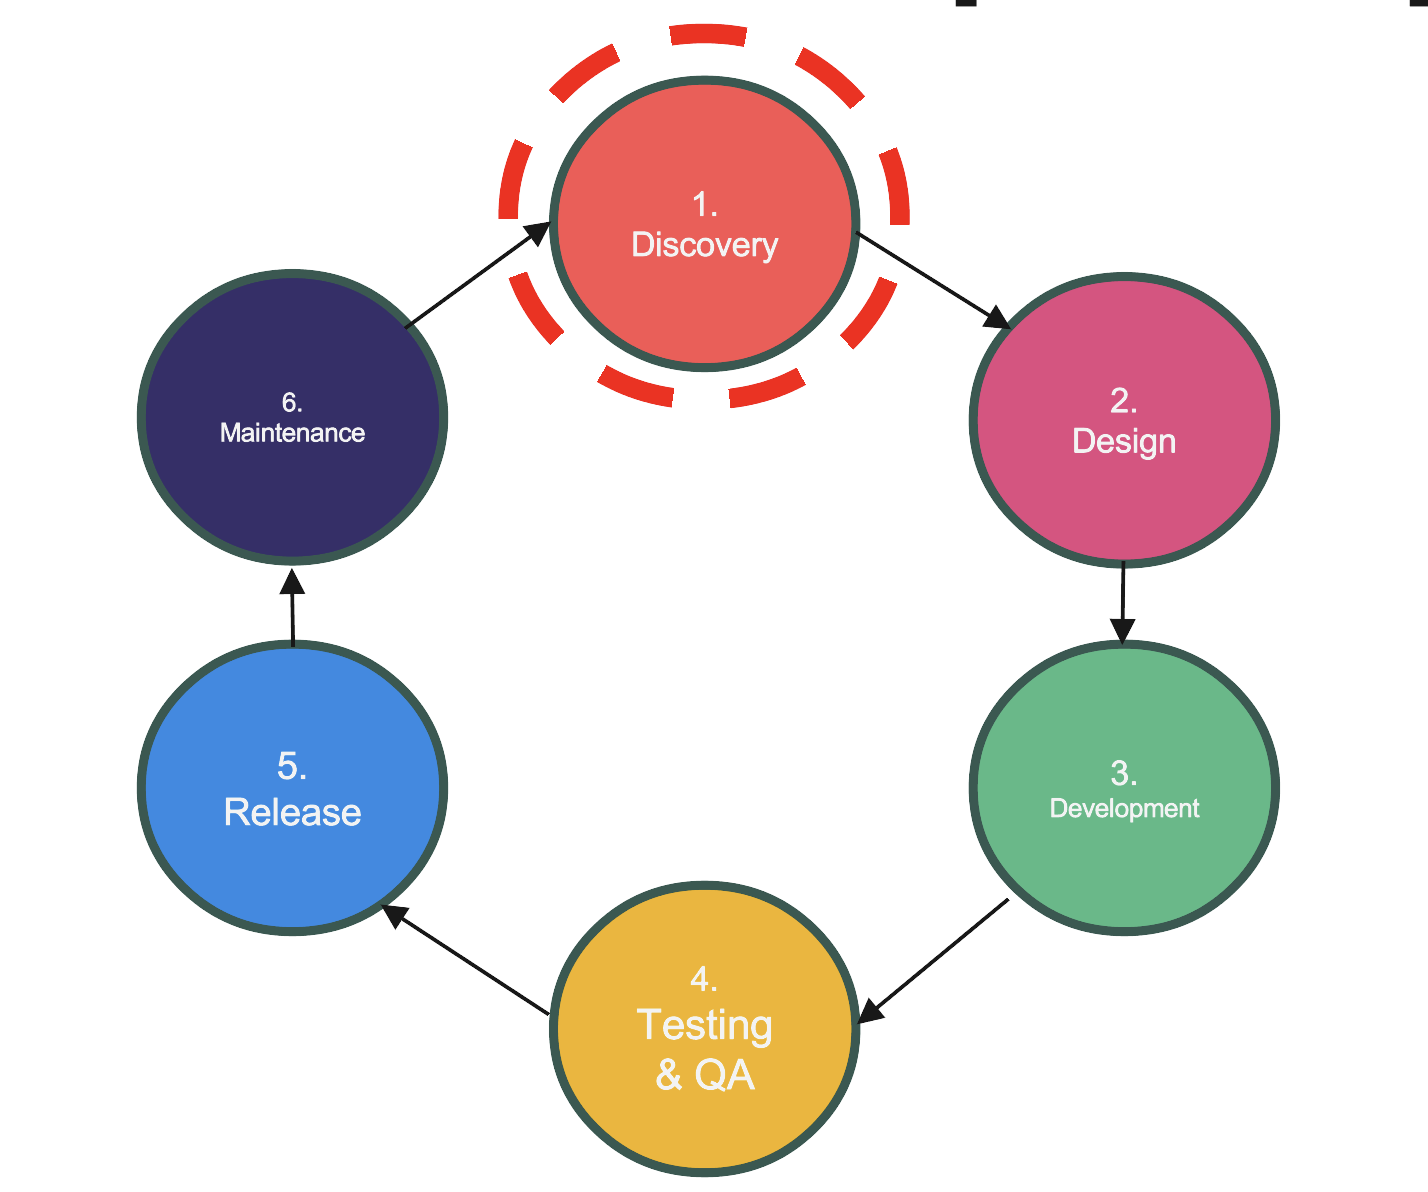
\includegraphics[scale=0.25]{/Users/juancamiloacosta/Documents/uniandes/tesis 2/thesis template repo/master-thesis-document/thesis-template/figures/software_process.png}
   			 \caption{The development process of a Software Application}
   			 \label{fig:ast}
\end{figure}


\section{Architectural design in software engineering}
For an effective and efficient software project development, we have to realize the respective investment in each stage. From the functional requirements creation to the design of each component and its features and constraints. To do this, it is necessary to make an architectural design. The architecture of a software project. In general, defines the components that require the entire system and the connections and relationships (and their types). Furthermore, each component has to be defined in this design. In that order, different standards ensure the system’s quality according to its architectural design.

\subsection{Architectural design in Android development}
Architectural Design in the mobile approach has been advancing step by step; this depends on the creation of new technologies in each development layer since the data management layer with the implementation of new database libraries like the room to the User Interface layers, with a different way of creating new screens inside the application (with the use of either JetPack Compose or Fragments organization).
Depending on what the simple should be, an application, how many components it would have, which of them would be connected, and the reasons for those connections. It is necessary to review different architectural patterns used recently and why we focus on one of them for architectural erosion detection.

\begin{itemize}
	\item MVC (Model View Controller): In this pattern, we divide the application components into the model, where we implement the connections with external platforms and internal data management. The controller component is used for setting the relation between the business logic and the User Interface (UI). The view component contains the UI. This pattern has been commonly used for the last 15 years due to its simplicity and popularity. However, the applications that use this pattern are very coupled, and their components depend strongly on others. It is usually found in business logic implementations and UI code fragments in the same code file, or data processing in business code components.  At the beginning of Android, architectural issues weren´t as important as they are today. If an Android application is simple in terms of realization, it is possible to use an MVC pattern.
	
	\item MVP (Model View Presenter): This pattern is managed in a different way than the MVC pattern in the relations between business logic and UI. In this case, we use a component named presenter to manage the events and behavior of each UI view or screen. This pattern is commonly used for single Applications that do not have scalability or application overloading. This pattern divides the presenter features connected with the UI features. The disadvantages of this pattern are related to a high coupling rate inside its components and a high complexity for managing the life cycles of an application. Furthermore, it is difficult to implement new feature development and maintenance for large-scale Android applications.
	
	\item MVM (Model View View-Model): This pattern is one of the derivatives of clean architecture, a concept widely developed in Backend and Frontend applications architectures. This pattern uses some concepts of clean architecture, like use case organization, when we implement a new feature in an independent way from others. With this pattern, we use reactive components. The application components use libraries like Dagger Hilt to implement the use of reactive data; this reactive data changes depending on a UI event. With the creation of the JetPack Compose framework. The JetPack Compose is based on reactive UI and is more declarative than the traditional form (the use of XML files and fragments structure for managing different application screens)
\end{itemize}

\begin{figure}
    \centering
    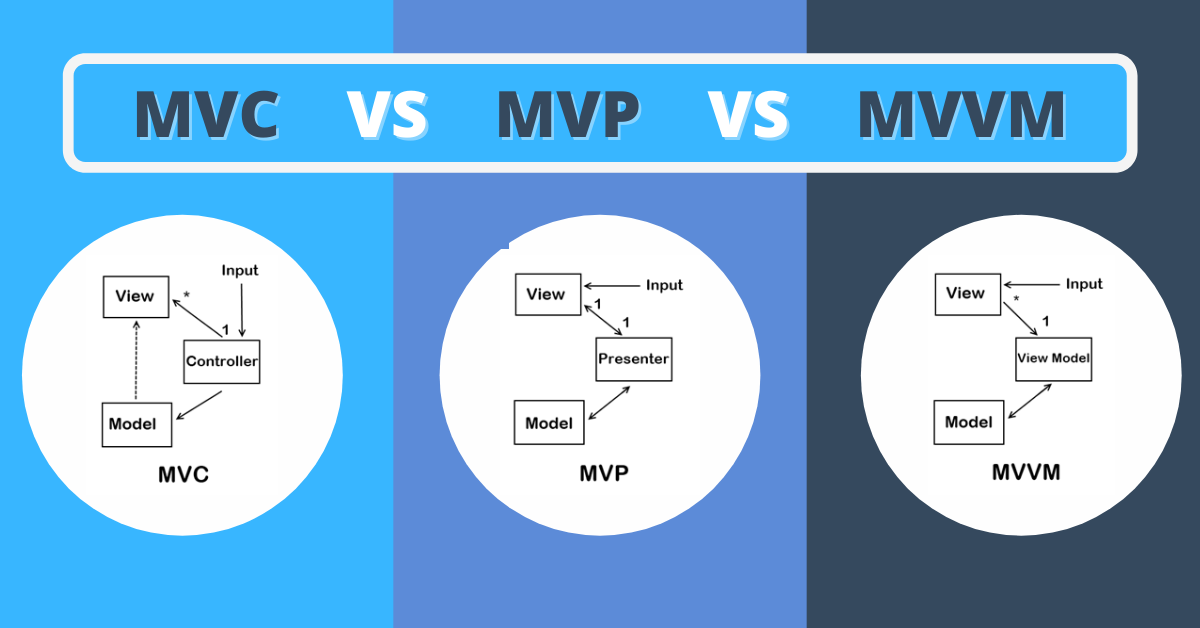
\includegraphics[scale=0.2]{/Users/juancamiloacosta/Downloads/thesis-template/figures/mvvm_mvp_mvc.png}
    \caption{Similarities and differences between Android architectural patterns. \citet{} }
    \label{fig:concept-map}
\end{figure}


In an Android application, it is not mandatory to use only an architectural pattern to achieve the functional and non-functional requirements of a software project. For example, it is very common to use the repository pattern declared in MVVM, divided into two: external connections and internal data management. Today, in the actual mobile development ecosystem, the most common framework that could be implemented with one or more architectural patterns is the three-layer pattern architecture: The UI layer, an optional layer named the Domain Layer, and the Data layer. Each layer could be or could not be, depending on each application's requirements. 

\begin{figure}
    \centering
    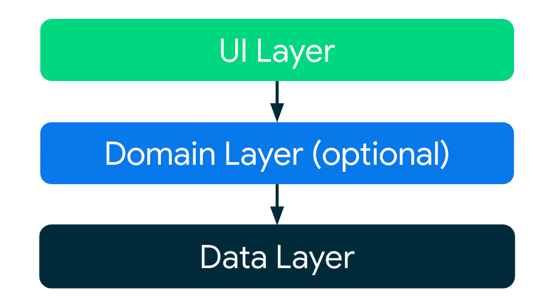
\includegraphics[scale=0.5]{/Users/juancamiloacosta/Downloads/thesis-template/figures/architecture_framework.png}
    \caption{Three-layer framework for mobile development. \citet{} }
    \label{fig:concept-map}
\end{figure}

The three-layer architecture will be used as the main architectural framework to realize this study with the MVVM architectural pattern. These patterns are the most used in modern mobile development and will give a first approach for how developers can detect and fix architectural violations in an Android application.

\subsection{Quality Attributes}
The consequences of the generation of architectural erosion could impact the different quality attributes contemplated. According to Bass \citet{bass-architecture-book}. There are six attributes based on ISO-25010. Those attribute qualities are:

\begin{itemize}
    \item Latency: This attribute measures the response time of the components according to the implemented architecture. Response times of each architectural component are very important.
    \item Scalability: Measures the ability of a system to grow in critical situations of system inputs. It is important for system availability when the user's connection rate increases.
    \item Security: Nowadays, a system must give protection to its users and their data, since the availability, integrity, and confidentiality of that data. This requirement is very important in the legal environment of a system.
    \item Availability: When the system can be available when a system failure occurs (it doesn't depend on the failure type). This quality attribute measures the time that the system takes to recover from a failure.
    \item Integration capability: Measures the ability of a system to integrate with other(s) systems (s), measures the time and effort that the system needs to make that integration in all its layers, from the data layer to the UI layer is necessary.
    \item Modification capability: Similar to the last quality attribute, it measures the time that the system needs to change one or more components inside its system. The effort measure could be many relationships (human resources effort, time costs, money costs, etc.)
\end{itemize}


\section{Architectural Erosion}
The Architecture Erosion concept was treated a long time ago. Since 1992, architecture erosion has had a formal definition, giving the relationship of this concept with architectural rules violations \citet{perry-wolf-reference}. It can be treated from different perspectives, from the violation of rules, structure, and quality to the evolutionary perspective. Furthermore, the concept has a strong relationship with other synonyms, like, for example, degradation. In another modern definition, architectural erosion is defined as the set of architectural violations that reflect the deviation of the implemented architecture from the intended architecture over time. In summary, in a more concrete definition, architectural erosion could be considered a phenomenon that reflects the deviation of an implemented architecture from the intended architecture in a software project.

\subsection{Approaches and Perspectives}
Due to the original concept of architectural erosion \citet{slr-base}. It could be studied and analyzed by different approaches:

\begin{itemize}
    \item Violation perspective: Denotes how the implemented architecture violates the design principles or main constraints of the intended architecture. These violations could occur in two phases: the design phase and the maintenance and evolution phase, making different changes step by step in the short and long term.
    \item Structure perspective: Where the structure of a software system encompasses its components and their relationships.
    \item Quality perspective: it refers to the degradation of the system quality, due to architectural changes that would generate architectural smells. It could include all the quality attributes contemplated in the industry.
    \item Evolution perspective: It shows the architectural inflexibility that increases the difficulty of implementing changes in the project and, therefore, decreases the sustainability of the system.

\end{itemize}

\subsection{Main Reasons and Symptoms }
Different factors could provoke architectural erosion in different stages of software project development. Due to these reasons, it is possible to make different solution approaches, and, therefore, the possibility of building different components based on those approaches. The main reasons found are:	

\begin{itemize}
    \item Architecture modularization: Due to the business needs, it is necessary to divide responsibilities between different components and layers in a software project. But sometimes it could produce non-functional components and deviate from the initial intended architecture.
    \item  Architecture complexity: if the intended architecture is very complex, it is possible to deviate from it the time goes by, producing the first symptoms of architectural erosion.
    \item Architecture size: Due to this attribute, and with no control over the maintenance of the software project, it is not possible to have good software maintenance for a long time.
    \item Design Decisions: If the design decisions during the initial stages of the project don't have enough support (like documentation, reviews, etc.), it could generate problems with the maintenance of refactoring of different components, decreasing the code quality and generating the first symptoms of architectural erosion.
    \item Duplicate functionality: As a consequence of the latest reasons too, duplicate functionality reflects the bad connection between layers of an architecture, and could be considered as the initial symptom of architectural erosion.

\end{itemize}
There are other reasons like bad documentation, bad programming features, but, in general, the main reasons were considered according to the architecture design stage issues.

\subsection{Consequences}
Are several points of view about the real definition of the consequences of architectural erosion violations inside a software project. The main problems that could generate the correct maintenance and the deviation from an intended architecture are:

\begin{itemize}
    \item Costs of software maintenance: Due to the lack no implementation of architectural erosion issues, this could affect one of the non-functional defined requirements, and after that, affect the actual software infrastructure.
    \item Software Performance: When one of the quality attributes is affected by the initial architecture design planning, it incurs a performance reduction of the intended architecture. In Android Apps, it could be more notorious, due to the limited resources of a mobile device, very different from a desktop device or server-type device.
    \item Software quality decrease: When architectural changes are made in a software project, it could affect the normal behavior of the application and, inside its source code, could imply bad code features implementation, decreasing the software quality, an important standard in a software project.
    \item Software Sustainability: The cost in terms of human resources, software infrastructure, time, money, etc, could increase if you do not attend to the architectural erosion insights in your software project, affecting non-functional requirements, and, in the long run, affecting the user performance.
\end{itemize}


\subsection{Metrics and treatments for architectural erosion}
Today. Some different metrics can determine architectural erosion in different approaches. According to \citet{ieee-erosion-metrics}. Some metrics have been created to analyze architectural decay in open-source projects, analyzing possible reasons, indicators, and solution strategies for it. In the resume, there are around 54 metrics that could determine architectural erosion in different stages, from the design stage to the deployment stage. Those metrics have been classified by measured artifacts, level of validation, usability, applicability, comparative analysis, and support tools. Different classifications could be implemented into a tool with a specific measure strategy for analyzing architectural erosion in any system.

\begin{figure}
    \centering
    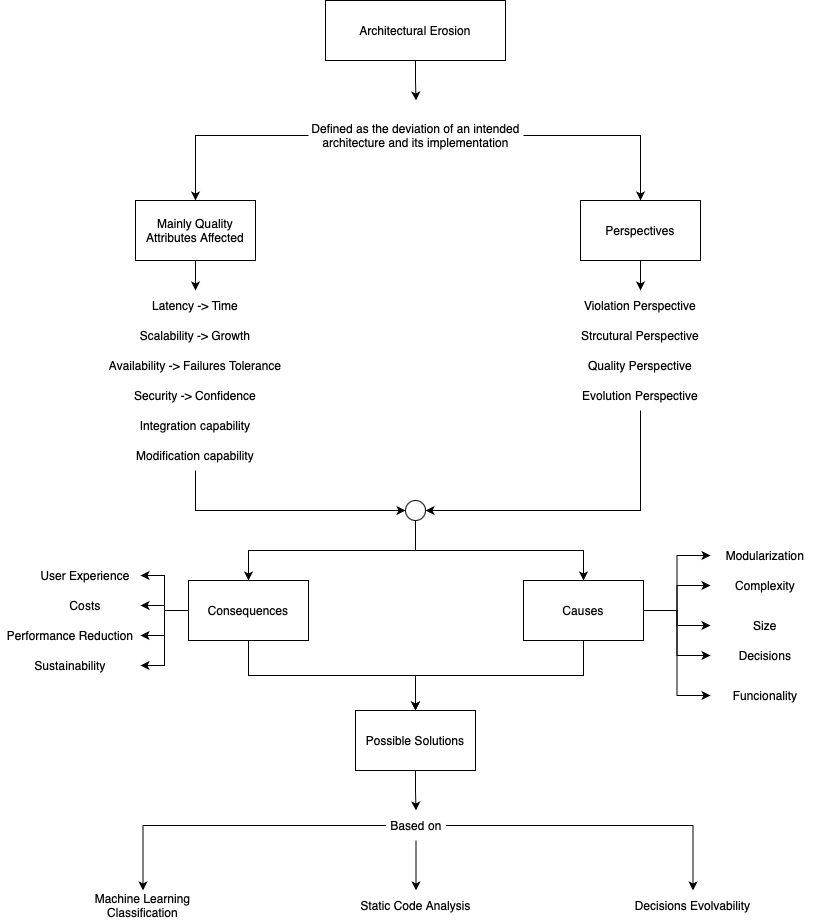
\includegraphics[scale=0.5]{/Users/juancamiloacosta/Downloads/thesis-template/figures/Architectural Erosion Concepts.drawio.png}
    \caption{Main Concepts of Architectural Erosion in Software Engineering }
    \label{fig:concept-map}
\end{figure}

\newpage

\section{Programming Languages fundamental for Software Analysis}
With the fundamentals of programming languages, it is possible to analyze the software building. Programming languages have a defined vocabulary, structure, and semantics. Those features make the use of AI tools and NLP techniques more effective. Furthermore, it is possible to create custom rules for checking a defined set of guidelines for a standard structure of different patterns in a software project. This is possible by detecting different semantical, grammatical, and lexical patterns inside the source code of any software project. In general, a programming language is defined by the following components:

\begin{itemize}
	\item Lexical component: In that component, we define the vocabulary and the set of words that will have a meaning for the programming language. For example, the word function in JavaScript programming language means a function declaration, or int in Java, which means the Integer primitive data type. It is necessary to define all the words that could be used in any source code file of that programming language.
	\item Grammatical component: With a defined set of words in the lexical component, the next step is to define the order in which words could be written in a code block. It is essential to define all the possible structures that could be defined in any program and the different ways that could be written. For example, most programming languages used in the industry have a defined structure of if statements and all the possible ways to write them.
	\item Semantical component: If we have a set of words and a defined order to write them, it is possible to build a kind of translator for a programming language. In this step, we define the type of translator with two options: for executable program building, that is, a compiler, one example of it is C language programming, and a semantic visitor that generates an executable program through a translation process between C code fragments and machine instructions. The other option is to make an interpreter, where, in execution time, we visit the line by line of code and translate it into a machine instruction; an example of that approach is the Python programming language. In both approaches, we specify the translation strategies mainly with two components: a visitor component and a call graph component.
		\begin{itemize}
			\item Visitor component: A visitor component consists of a structure built from grammatical and lexical components of a programming language. In that structure, we can find how all the statement code blocks are defined in all source code files of a software project. We can find the name of every parameter declared in any function and the name of any class of any code statement defined in any source code file. With this component, we can detect any pattern in names and data types inside all code fragments and combine them for more customized check rules (security issues, connectivity issues, and others).		
			\begin{figure}
    				\centering
    				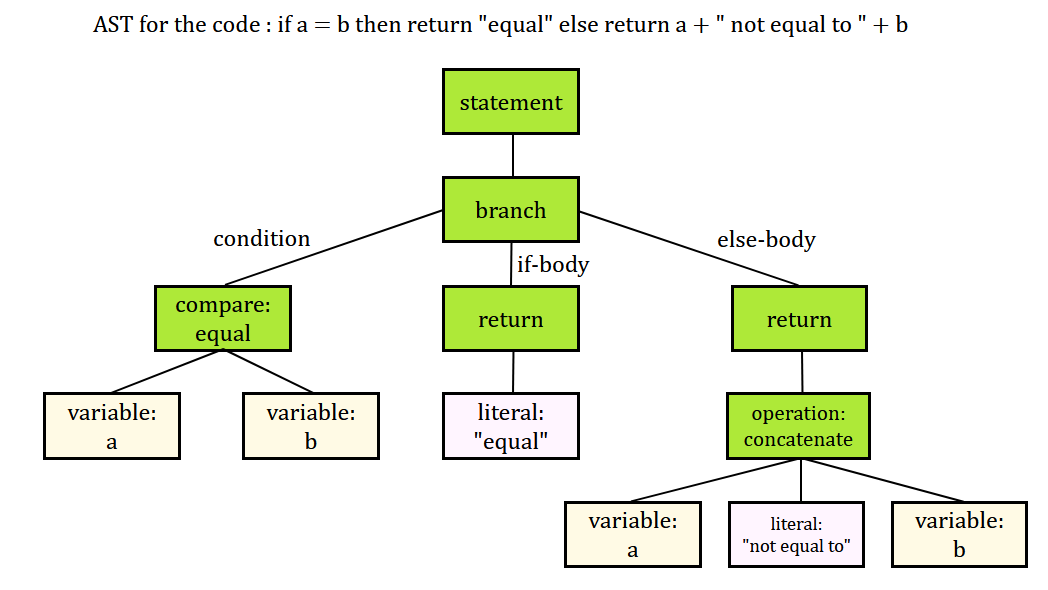
\includegraphics[scale=0.5]{/Users/juancamiloacosta/Documents/uniandes/tesis 2/thesis template repo/master-thesis-document/thesis-template/figures/abstract-syntax-tree.png}
   				 \caption{Example of an Abstract Syntax Tree (AST) statement. \citet{} }
   				 \label{fig:ast}
			\end{figure}
			\item Call Graph component: The call graph component is very similar to the visitor component. The main difference is that we can find all the dependency relationships between all the source code files of a software project. With this dependency structure, we can detect the high dependency between components and their high coupling rate.
			\begin{figure}
    				\centering
    				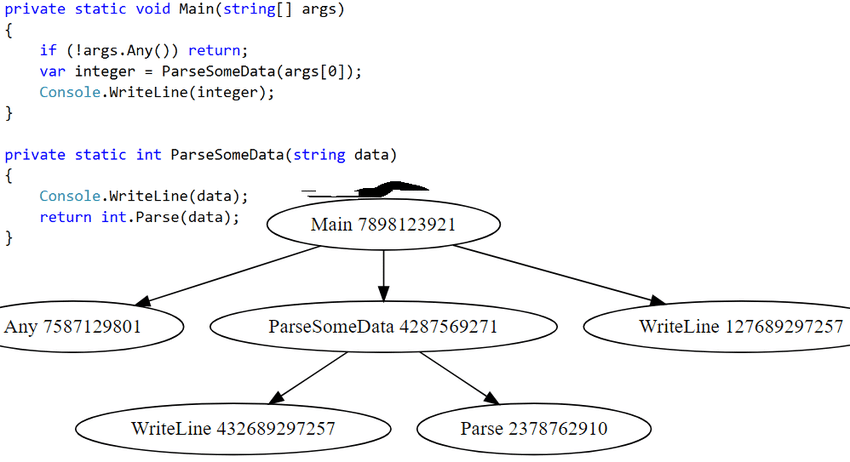
\includegraphics[scale=0.5]{/Users/juancamiloacosta/Documents/uniandes/tesis 2/thesis template repo/master-thesis-document/thesis-template/figures/Call-graph-in-C-source-code.png}
   				 \caption{Example of an Abstract Syntax Tree (AST) statement. \citet{} }
   				 \label{fig:ast}
			\end{figure}
		\end{itemize}
\end{itemize}

With all the programming language components and the way of translating it to machine instructions, it is possible to make custom check rules for different violations detection to different standards. In architectural erosion detection, these concepts will be fundamental.

\section{Representative set of a sample}
In statistics, several sampling methods are effective in selecting criteria; each alternative has a way for selecting data randomly that represents a minor scale all the entire dataset. One way is to select a representative set from the original population. In this case, it is possible to make a weighted-random selection of some individuals from any population that represents the main features of all population \emph{reference representative set}

\section{Natural Language Processing in Software Issues Detection}
Before solving architectural erosion insights into a software project, you have to detect the real violation types that could appear in your software project. There are some approaches for software issue detection using actual natural language processing methodologies that have been powered with Machine Learning Techniques. Natural Language Processing (NLP) gives the ability to extract relevant information from large text sets known as a corpus. Nowadays, NLP is very useful for many tasks, like text generation or classification. Even with a different approach, the NLP actual tools have had a better performance of the same tasks in code due to their standard structure, which does not present different language variations that could be present in a spoken language.

NLP has a set of different preprocessing methods for language models. Due to the complexity of text representation for computer processing, it is necessary to define a standard input structure for a model language. Before this, you have to make a series of processes for getting the standard structure of a given corpus of text. The process that enables those actions is named text normalization \citet{nlp-fundamentals}. With the use of regular expressions, you could build a dictionary of words, which is useful for getting a standard structure and enabling the text words for the modeling task. The main stages and processes for the dictionary building are:

\begin{itemize}
    \item Tokenization: Given a character sequence, in this case, a sequence of words of a given context, you can split that sequence into minimal processing units named tokens. These tokens are normally defined in terms of words. These tokens will create the base dictionary to begin the text processing into a language model \citet{information-retrieval}. 

    \begin{figure}[H]
    \centering
    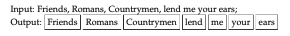
\includegraphics[scale=0.5]{/Users/juancamiloacosta/Downloads/thesis-template/figures/tokenization.png}
    \caption{Tokenization process of one sentence \citet{information-retrieval} }
    \label{fig:tokenization}
    \end{figure}
    
    \item Removing Stop Words: In the basic language modeling tasks, it is necessary to remove words that do not have relevant semantic information inside a text or a text corpus; those words are named Stop Words. Stop Words are words that do not contribute to the meaning of a sentence, like prepositions, articles, etc. In actual language models (Large Language Models), it is very important to maintain Stop Words to get a better specific context for next-word prediction or sentence classification. There are different strategies for removing those words; the most common is removing by collection frequency, due to the number of appearances in the corpus, which is enormous compared with relevant words. In document retrieval, the rare words are the most important for giving an efficient model over the text corpus \citet{information-retrieval}. 
    \item Lemmatization: For new tokens controlling and token derivations, it is essential to create tokens from the roots of the words, to reduce inflectional forms and related forms of words with the same root. In some cases, it is difficult to implement that process because you must have a root word dictionary to get root tokens. In this case, in different contexts, could generate conflicts for getting roots of specific context words \cite{information-retrieval}.
    \item Stemming: This process consists of a heuristic process to cut off some characters at the end of each word, reducing the derivation of some words, with the same objective as the lemmatization process. In English, language could be an efficient technique, but it could have some conflicts with other languages.
\end{itemize}


\subsection{Word Embeddings for Word Representation}
As said in the last section, language models need to have a numerical representation of the corpus text for modeling tasks. To solve this, you must define a standard structure based on the decided model inputs. The most common structure is a word embedding representation, where you define a numerical vector to represent a specific context (where the embedding was trained) for use as input into a language model. This representation gives all model vocabulary a vector representation, where you can observe similar words, different words, and how much distance is between them. This representation is useful for similarity word management and getting the relationships between different features inside them \citet{nlp-fundamentals}. 

    \begin{figure}[H]
    \centering
    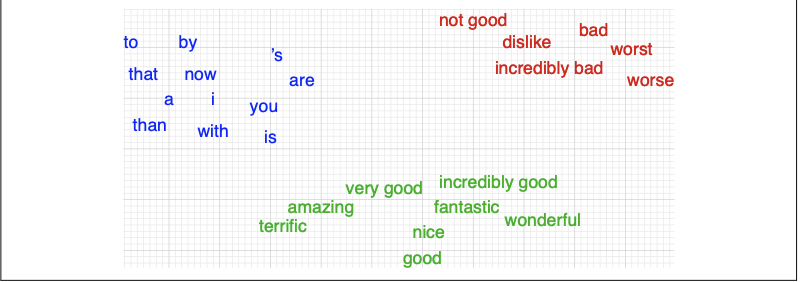
\includegraphics[scale=0.5]{/Users/juancamiloacosta/Downloads/thesis-template/figures/word_embedding_representation.png}
    \caption{Representation in two dimensions of Similar Words gives a Word Embedding \citet{nlp-fundamentals} }
    \label{fig:word-embedding}
    \end{figure}

\subsection{Performance and Similarity Metrics in NLP}
Maintaining and defining an objective in terms of performance is very important. Different metrics represent the behavior of a classic or modern language model based on next-word probabilities (like the anagram model when you generate an n-tuple of words and calculate the occurrence probability of that word sequence). For information retrieval, when you, in the same case of word embedding representation, have a vector representation, you must use a metric based on the vector's components. In the same dimension, you could determine the similarity between two vectors and verify the semantic similarity between two words in an NLP context. One of the most used metrics in this approach is cosine similarity. This metric combines the product of the two vectors and the difference between their components. The Similitude Cosine metric is defined as:

\begin{equation}
cos(v,w) = \frac{v.w}{|v||w|} = \frac{\sum_{i=1}^{N} v_{i}w_{i}}{\sqrt{\sum_{i=1}^{N} w_{i}^{2}} \sqrt{\sum_{i=1}^{N} v_{i}^{2}}}
\end{equation}

With this metric, we can conclude the similarity between two words (or two documents without another research context). If the similarity value is high, the words can be considered similar.

\section{AI models and Software Engineering}
With the mentioned NLP fundamentals, different machine learning models have been built from software engineering quality processes, like code refinement, code quality processes. and code generation with better performance compared to the given source code from any software project. All the machine learning models have a basic component that enables their computational processing. This component is a neuron, a mathematical model of a neuron of the human brain. The neuron is the basic processing unit that, through a regression model and an activation function for learning different patterns from the input dataset, depending on the determined learning task for the model. With layers of a series of neurons, it is possible to build a neural network for learning complex patterns from the input data.
With that concept, different basic models have been built for different learning tasks:

\begin{itemize}
	\item Logistic Regression: The logistic Regression model is a machine learning model that acts a the processing unit of a deep neural network. Logistic Regression is a supervised machine learning algorithm for classification tasks based on linear regression and gives a probability that any data belongs to any output category. First, we use linear regression with all the data features. After that, we use a function like the sigmoid function to get the probability of each data row. The Logistic Regression could vary depending on the output classes (binomial or multinomial).
	
	\begin{equation}
		z = w_0 + w_1*x_1 + w_2 * x_2 + ... + w_n*x_n
	\end{equation}
	\begin{equation}
		\sigma = \frac{1}{1 + e^{-z}}
	\end{equation}
	\item Decision Trees: The Decision Trees model is a model that tries to build a tree structure for predicting the class of any data input. Asking about every feature of every row of data, it classifies depending on the achievement of any feature or not. The main disadvantage of this model is the tendency to overfit and a poor performance with very different data compared to the training data.
	\item Perceptron model: With the concepts from the Logistic Regression model, the perceptron model is built. The perceptron model acts as a simple human neuron, with the use of linear regression and any activation function like the sigmoid function or the ReLu function, that classifies the input data into the output classes
	\item Deep Neural Network: With the concept of neuron extracted from the perceptron model, a new model can be extended. The neural network model is the basic Deep Learning model. The neural network model collects a set of neurons that act as the basic processing units and "learn" the main features of the input data in the training phase (validation data is recommended for this kind of model). Deep Neural networks allow for more complex data as images and multimedia files. This kind of model is the starting point for building more complex models and architectures. For learning tasks related to natural language, it needs an attention mechanism is needed for handling the main features based on the context of any text corpus.
\end{itemize}


Despite the accuracy of those models for some learning tasks. They have any disadvantages for more complex and structured data. With the fundamental concepts, it is possible to build more complex machine learning models according to more complex learning tasks and their data input structure. One of these kinds of models is the models are based on the Transformers architecture.

\subsection{Transformer Architecture}
Some architectures of machine learning models use an attention mechanism to get the main features of a large amount of data in natural language. The first one is the Long Short-Term Memory (LSTM), which holds some features of data from previous learning steps. This kind of model is used for learning tasks of input data that depends on previous data in the learning stage. However, the LSTM model does not hold the features of a large text corpus or many previous steps. Furthermore, the LSTM models demand a high rate of computational resources in terms of memory and computing processing for training the model based on the previous steps or previous data. To optimize that model, in attention is all you need, the Transformer architecture model is proposed \cite{attention_is_all_you_need}.

The Transformer architecture uses attention heads as an attention mechanism named the attention heads. An attention head uses three matrices that act as three roles: the query matrix, the key matrix, and the value matrix. Every matrix helps to retain all the important information from many previous steps. The Transformer architecture uses a normalization layer and a feed-forward layer for mixing the positional encodings of the input data with the result of the processing of the heads' attention component. Another component is the Word 
An embedding model that combines a positional encoding to consider the information in the input data.
The Transformer architecture is the basic model for building the actual Large Language Models (LLM) and derived models for specified learning tasks, like encoder-only models for classification tasks, decoder-only for generation tasks, and the autoencoder models that combine classification and generation learning tasks.
In software engineering, it will be useful for developers' message treatment for bug and code smell detection, and for source code treatment.

    \begin{figure}[H]
    \centering
    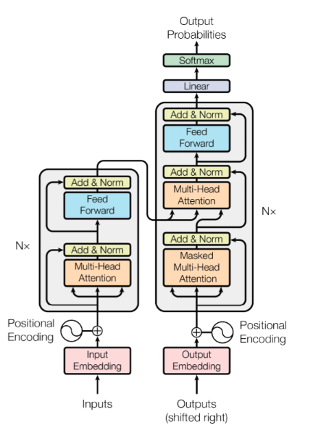
\includegraphics[scale=0.5]{/Users/juancamiloacosta/Documents/uniandes/tesis 2/thesis template repo/master-thesis-document/thesis-template/figures/transformers.png}
    \caption{the Transformer architecture for machine learning models \citet{attention_is_all_you_need} }
    \label{fig:word-embedding}
    \end{figure}

   






